\begin{figure}
  \centering
  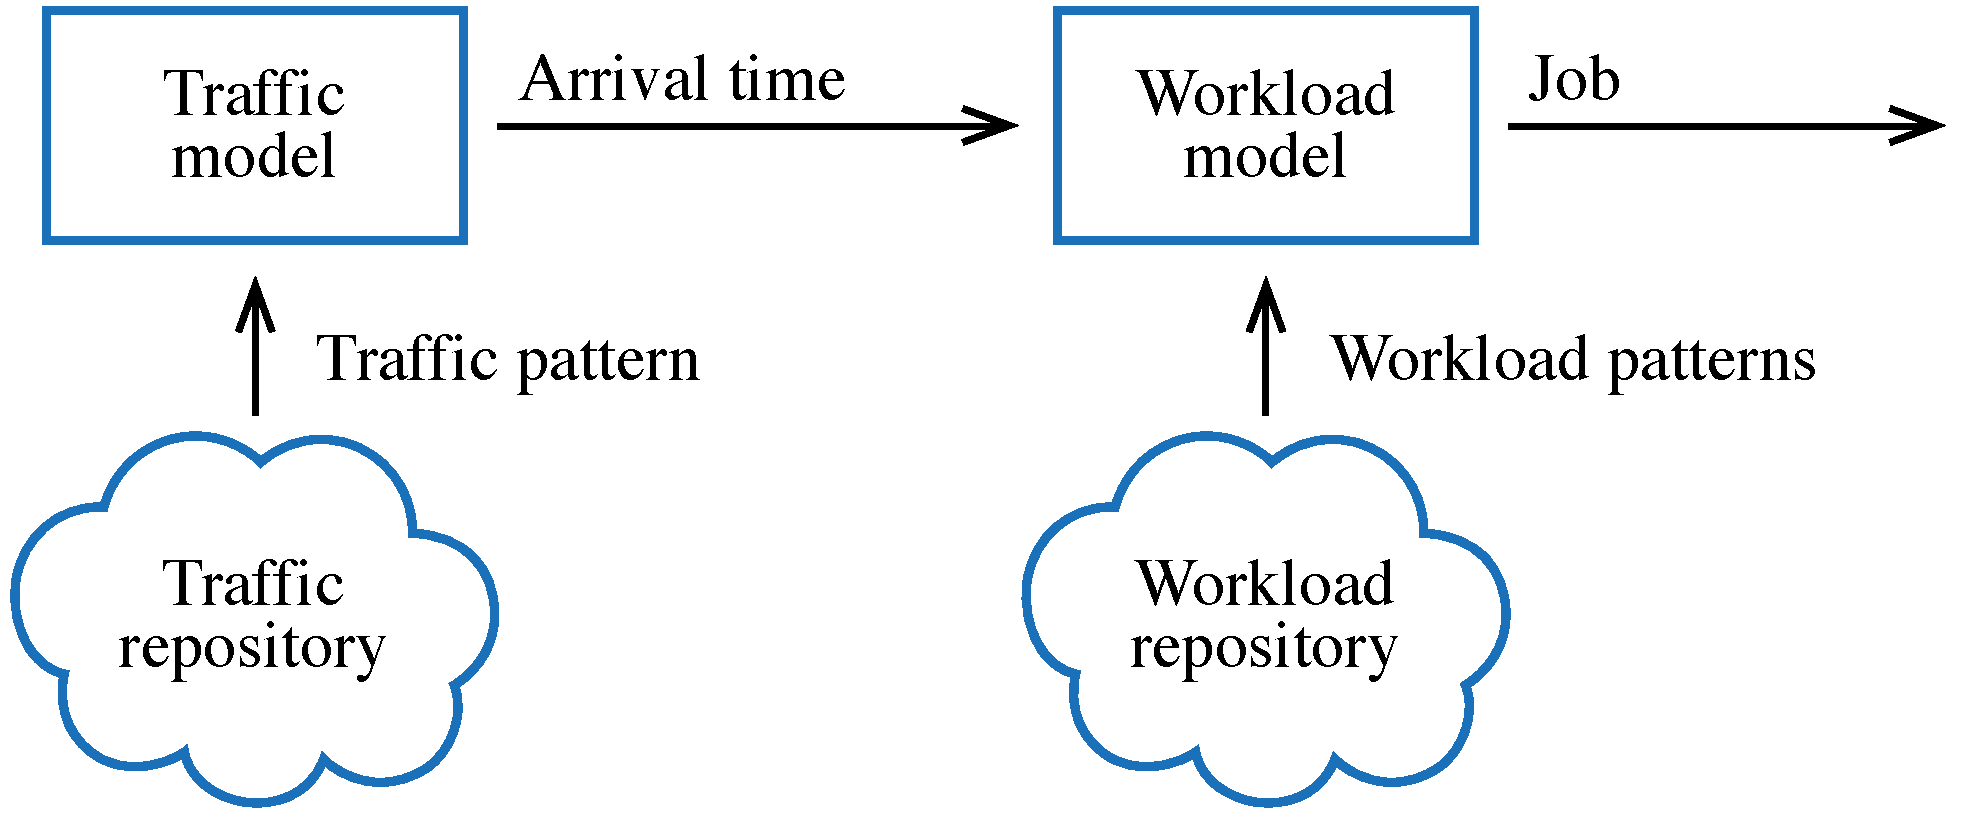
\includegraphics[width=1.0\columnwidth]{include/assets/figures/streams.pdf}
  \caption{The stream of arrival times and the stream of jobs. Each job is
  characterized by an arrival time and a workload.}
  \flab{streams}
\end{figure}

In the previous subsection, we introduced our approach to generating streams of
arrivals; however, an arrival is only a time stamp without any information about
the actual workload. In this subsection, we describe how workload candidates are
obtained and utilized for substantiating job arrivals, which is depicted at the
bottom of \fref{methodology}. Figure~\ref{fig:streams} might also be helpful to
clarify the relation between the previous and current sections. To begin with,
workload candidates should conform to a number of criteria. First, since we aim
to produce realistic power and temperature trace, workloads should represent
well the applications or services that the system in question is supposed to
provide to the end user. Second, a workload should be fast to evaluate, which,
in our context, refers to obtaining the power consumption over time of that
workload.

Our workload modeling is based on full-system simulations of reference programs.
However, if we had incorporated such simulations into our workflow
\emph{directly}, we would have wound up with a configuration similar to the one
displayed in \fref{development}. This, of course, would have defeated the
purpose of our work since, as motivated in \sref{simulation}, detailed
simulations are too time consuming. Instead, we propose the use of high-level
recordings; this functionality corresponds to the modules labeled ``Recorder''
in \fref{methodology}. To elaborate, using an adequate simulator capable of
modeling the target architecture, we execute each reference program in isolation
and record certain information about this execution.\footnote{Such a technique
is similar in spirit to PinPlay \cite{patil2010}, which is a tool for recording
and replaying an execution of a program at the instruction level.} At a later
stage of our pipeline (see the Streamer module in \fref{methodology}), the
collected information is utilized in order to flesh out jobs upon their arrival,
and this stage requires no simulation. These recordings are building blocks:
they are combined to form complex workloads corresponding to multiple programs
running in parallel, which will be elaborated on in \sref{composition}.

From our experience, performance and power simulation takes by far the largest
expense in terms of time. Therefore, the information about a reference program's
execution that we propose to record is the power consumption of that execution.
This approach pushes the aforementioned expense to the data-acquisition stage
and eliminates it all together from the data-synthesis stage. To put it
differently, each recording is obtained via a one-time simulation at the
data-acquisition stage, and from there on the recording is reused as many times
as needed at the data-synthesis stage of our methodology. Since the actual data
generation, which takes place at the data-synthesis stage, is deliver from the
expensive simulations, it has a very low computational demand. This demand is
negligible compared to the one of the scenario depicted in \fref{development},
in which one undertakes performance and power simulations nonstop.

The power consumption of a program can be recorded differently; let us be more
specific about what we do. The first aspect to note is that we record power as a
function of time (assuming a certain sampling interval). Second, the dynamic and
static components of the power consumption are recorded separately in order to
get a better control over the subsequent composition (\sref{composition}).
Third, the power consumption is recorded for all processing elements that are
relevant to the subsequent study (for instance, cores and shared caches).

The result of the recording procedure is a repository of power traces
corresponding to real programs, which we refer to as workload patterns; see the
clouds in \fref{methodology} and \fref{streams}.

Full-system simulations obviously take time; however, as mentioned previously,
they should be done only once. Moreover, since researchers tend to test their
ideas using similar sets of benchmark suites, such as \sc{PARSEC}
\cite{bienia2011} and \sc{SPEC CPU2006} \cite{cpu2006}, and considering similar
sets of target architectures, it is reasonable to create a common repository of
power patterns that will be populated and maintained online by the research
community. The repository could be structured in a way that would allow for a
proper accommodation of different recording conditions. Having established such
a common repository, power patterns will be at a one-click distance from any
single researcher, and no prior simulation will be needed. The role of the
repository could be similar to the one played nowadays by the benchmark suites
themselves, but it would be on a different level of abstraction and for a
different purpose.

Let us now turn to the question: How do we choose which workload pattern to use
for a particular arrival? In \fref{streams}, this functionality resides in the
top-right module referred to as the workload model. The input to this model is a
stream of arrival times, and its output is a stream of fully characterized jobs
(time and work). The logic of the workload model can be dependent on the input
stream and introduce autocorrelations to the output stream, which allows for
modeling, for instance, periodic and/or coupled workloads. Since such aspects
rely heavily on domain-specific knowledge, we refrain from providing any
particular dependency model. The default option that is used in our toolchain
(to be discussed in \sref{toolchain}) for assigning workloads to job arrivals is
drawing samples from a uniform distribution over a set of workload patterns.
This default behavior can be adjusted as needed for the problem at hand.

An optional job of the workload model is a set of workload transformations. A
workload transformation is an operation that can be used for workload
diversification and for emulation of the effects of such techniques as dynamic
voltage/frequency scaling. A job (with a workload selected) can pass through a
number of filters---such as noise, offset, scale, stretch, and shrink---before
being pulled from the job stream. This, however, should be done thoughtfully as
the purpose of recording power patterns is in part to bring in realistic power
fluctuations.

To recapitulate, we have obtained a database of reference workloads and
discussed the formation of job streams from arrival streams (\fref{streams}).
The patterns correspond to executions of real programs and, thus, exhibit
realistic traits.
